\section{Temporal models, concepts and operators} \label{tconcepts}
The SAX transformation procedure described in the previous section yields symbolic time-series based on the real-valued data. Having such a symbolic representation (also called in the literature as a \textit{symbolic temporal data}) is very advantageous comparing to the real-valued data due to the vast amount of the algorithms developed for the string processing. In following subsections we will review up to date work in the mining of tempral symbolic data defining symbolic temporal data models, temporal concepts and operators.

\subsection{Temporal data models} \label{tconcepts_models}
Fabian M\"orchen in his report \cite{citeulike:1748833} aggregated many work in the field of data mining from symbolic temporal data. Two figures taken from this work (Figure \ref{fig:concepts1}) depict a hierarchy of time-points (left panel) and time-intervals (right panel) data models, concepts and operators.

\begin{figure}[tbp]
   \centering
   \includegraphics[height=45mm]{concepts1.eps}
   \caption{The temporal concepts and operators from \cite{citeulike:1748833} for both: time point and time interval data models.}
   \label{fig:concepts1}
\end{figure}

While the time-points data model is intuitive and resembles the actual real-valued time series, the time intervals temporal data model is built upon the concept of \textit{duration} which is a repetition of the property over several time-points. \textit{Time-intervals} are continuous groups of discrete time instants and some algorithms and applications operate with this data type rather than individual points. Time-intervals essentially are sets of two or more continuous points and two successive time points define a minimal interval which starts at the earlier point and continues to the latter point inclusevily. Allen \cite{citeulike:191348} says: ``In English, we can refer times as points or as intervals...'' giving next two examples: ``We found the letter at twelve noon.'' and ``We found the letter while John was away.'' pointing that there are temporal relations involved.

\subsection{Temporal concepts} \label{tconcepts_concepts}
The concept of \textit{concurrency}, as described by M\"orchen, explains the closeness of two time-points in time without considering their ordering, - a coincidence of events in time is the most important property. The \textit{synchronicity} is a special case of concurrency where events occur synchronously in time.

The \textit{order}, and \textit{synchronicity} concepts in the Time intervals model are analogous ones in the Time points model, whether the Time intervals \textit{coincidence} describes an intersection of intervals in time.

\subsection{Temporal operators} \label{tconcepts_opertaors}
The time point operators from the Figure \ref{fig:concepts1}: \textit{before}, \textit{after} and \textit{equals} precisely define the relation of points in time. The \textit{close} operator is a ``fuzzy extension for temporal reasoning'' since it encapsulates other three. Note that some threshold can be used to relax or constrain these operators, for example we can consider points equal to each other even if they are less than $k$ time units apart.

The Time intervals operators a more complex and were examined in many work. In 1983 Allen \cite{citeulike:191348} proposed thirteen basic relations between time intervals which are distinct, exhausting and qualitative. In his work Allen showed that thirteen relationships are sufficient to model the relationship between any two intervals. Figure \ref{fig:allen} depicts Allen's relations. This relations and operations on them are forming \textit{Allen's Interval Algebra}.

Despite the exhausting property of Allen's relations, while working on the multimedia data analysis, Snoek \& Worring \cite{citeulike:272197} discovered two practical problems: first is that ``in video analysis, exact alignment of start- or end- points seldom occurs due to noise... '' and the second is that ``two time intervals will always have a relation even if they are far apart in time...''. In order to resolve these issues authors had to relax a set of Allen's relations and introduce a new \textit{NoRelation} relation. This new relaxed set of 14 relations named TIME (Time Interval Multimedia Event) was built with two time-interval parameters: $T_{1}$ for the neighborhood in which impresize boundary segments considered synchronous and $T_{2}$ which assigns two intervals as \textit{NoRelation} if they are more than $T_{2}$ time apart.

\begin{figure}[tbp]
   \centering
   \includegraphics[height=20mm]{allen.eps}
   \caption{The Allen's thirteen basic relations (from \cite{citeulike:4072008}) sorted by the degree to which $a$ begins and later ends before $b$. All but \textit{equals} can be inverted.}
   \label{fig:allen}
\end{figure}

Freksa \cite{citeulike:4991332} proposes even more general approach for interval reasoning based on the relations between semi-intervals arguing that  ``semi-intervals are rather natural entities both from a cognitive and from a computational point of view''. Freksa introduces ten operators, Figure \ref{fig:freksa}, which fully exploit incomplete inferences and knowledge about events: ``... we may know that a certain event $Y$ did not start before a given event $X$, but we do not know if $X$ and $Y$ started simultaneously or if $Y$ started after $X$.'' This approach easies representation of incomplete knowledge
by simpler formulas instead of long disjunctions of Allen's algebra. Two intervals can be related by their start points with \textit{younger}, \textit{older} and \textit{head to head} operators. The operators \textit{survives}, \textit{survived by} and \textit{tail to tail} are defined by using end points of each interval. Based on the relation between a start point of one interval and an end point of the other \textit{precedes}, \textit{succeeds} and \textit{born before death of} with inverse \textit{died after birth of} operators defined.

Freksa combined basic operators introducing \textit{contemporary of} relation, \textit{younger contemporary of}, \textit{older contemporary of}, \textit{surviving contemporary of}, \textit{survived by contemporary of}, \textit{older \& survived by} and \textit{younger \& survives}. 

Rainsford \& Roddick in \cite{citeulike:5000685} implemented a system of temporal knowledge discovery based on the Freksa's relations. Later, Roddick introduced \textit{Midpoint Interval Operators} extending Allen's and Vilain's \textit{five-points} \cite{citeulike:5000906} relations with nine different \textit{overlaps}. Two overlaps \textit{large overlap} and \textit{small overlap} depicted at the Figure \ref{fig:freksa} panel $b$. This improvement allowed the handling of coarse temporal data and data from streams.

Further extensions were proposed by M\"orchen \& Ultsch in the form of UTG (Unification-Based Temporal Grammar) introducing an extension to the Allen's \textit{equals} operator with \textit{more or less simultaneous} and \textit{coincides} operators as shown at the Figure \ref{fig:freksa} panels $c$ and $d$. Later, the Time Series Knowledge Representation (TSKR) hierarchical language for expressing temporal knowledge in time interval data was built by the same authors on the base of UTG \cite{citeulike:3978065}. 
It was shown that TSKR, while compared to other alternative approaches, has advantages in robustness, expressivity, and comprehensibility

\begin{figure}[tbp]
   \centering
   \includegraphics[height=70mm]{freksa.eps}
   \caption{Panel a): Freksa�s semi-interval relations between the intervals $A$ and $B$ with inverse operators in italics. Panels b), c), d): Alternative interval operators.}
   \label{fig:freksa}
\end{figure}
